

\begin{frame}
\frametitle{Multiple Shooting}
\only<1>{
% Bild von Johannes einfügen was Multiple shooting zeigt OHNE Steuerung
}
\only<2>{
% Bild von Johannes einfügen was Multiple shooting zeigt MIT Steuerung
}
\only<3>{\begin{figure}
\centering
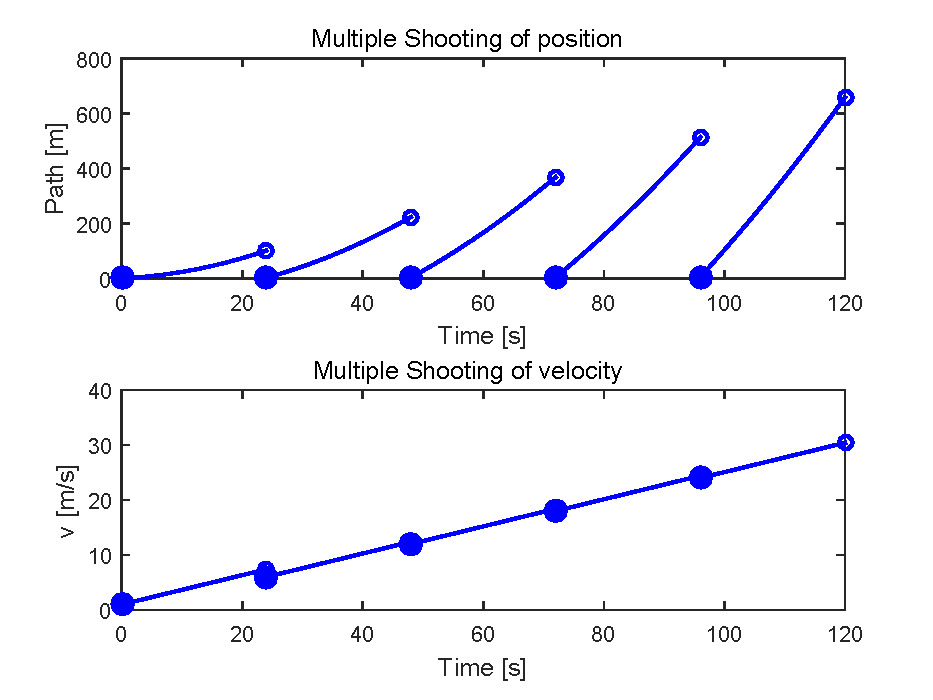
\includegraphics[width=0.9\textwidth]{Sabina/MultipleShooting21.pdf}
\end{figure}}
\only<4>{\begin{figure}
\centering
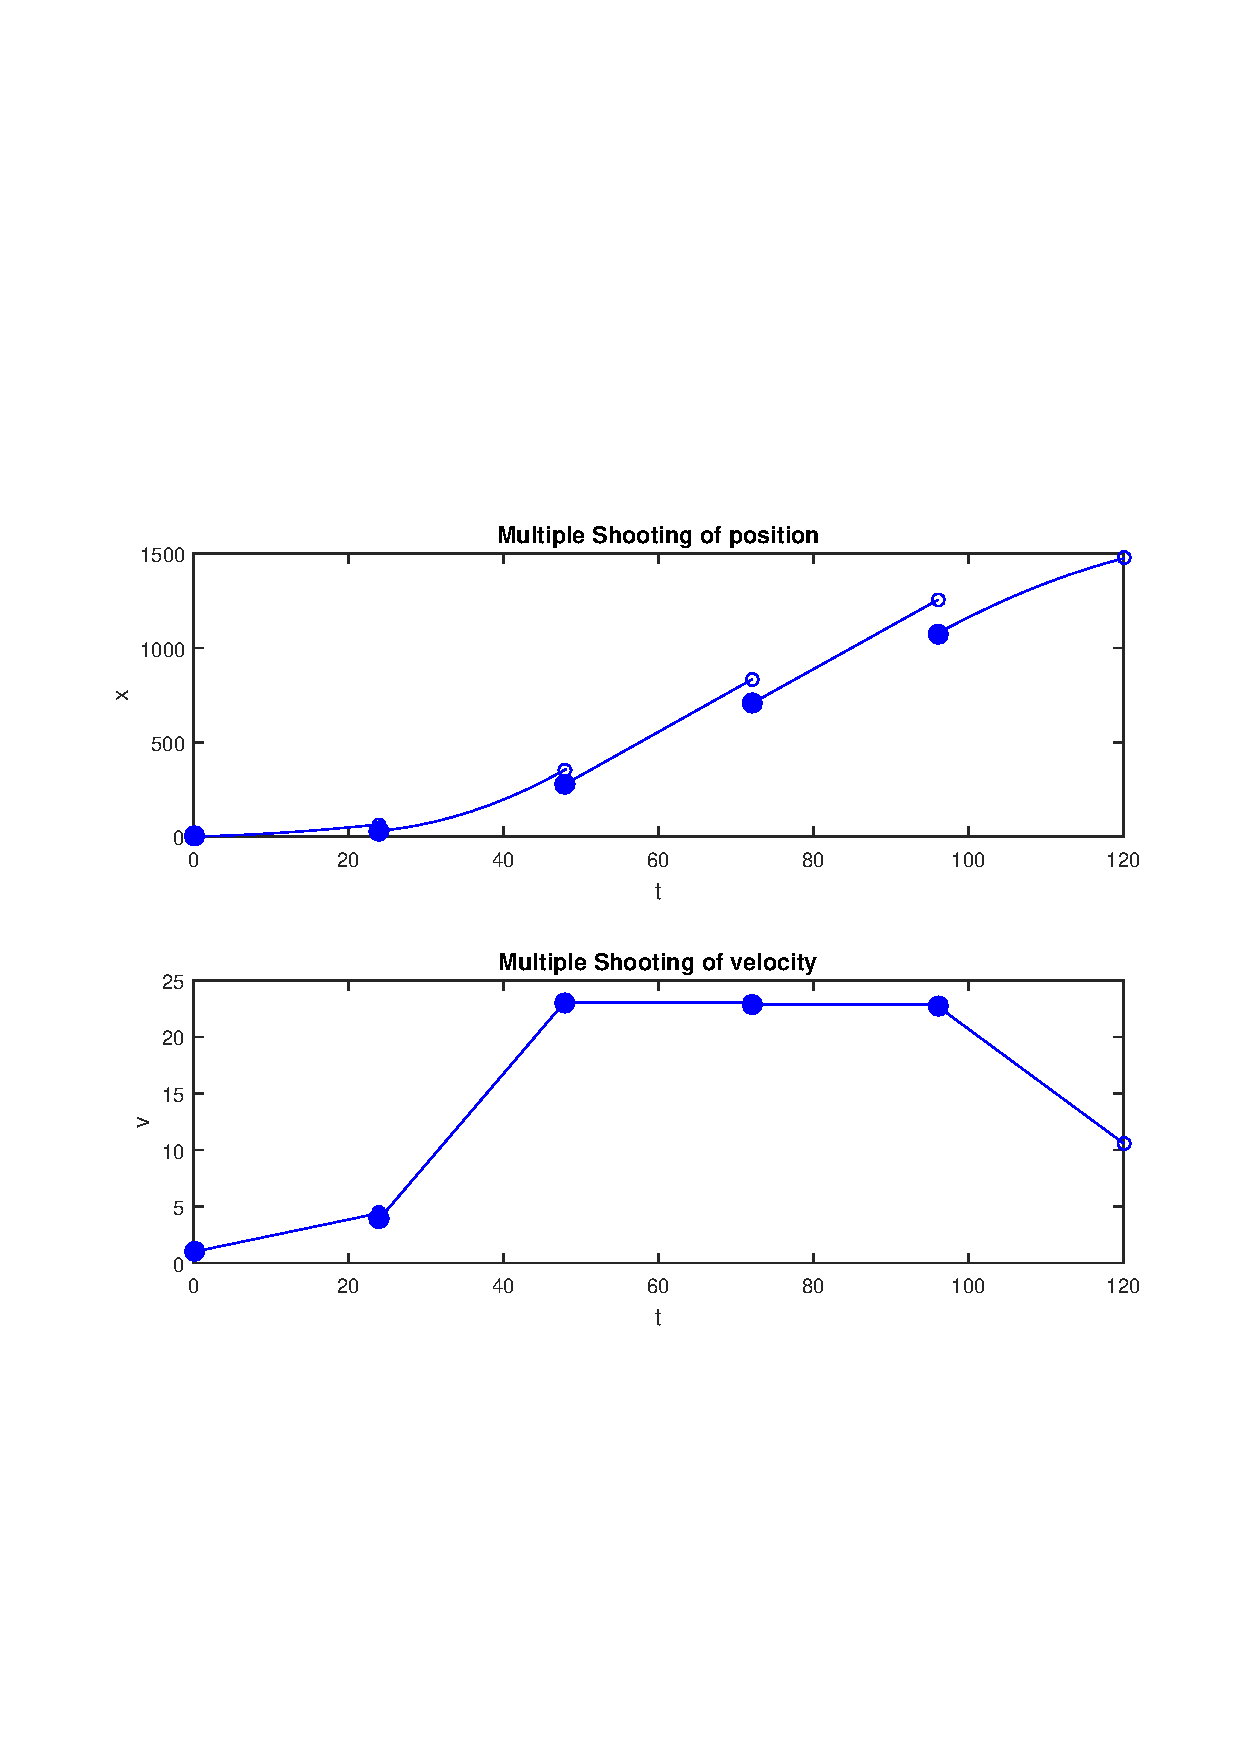
\includegraphics[width=0.9\textwidth]{Sabina/MultipleShooting24.pdf}
\end{figure}}
\only<5>{\begin{figure}
\centering
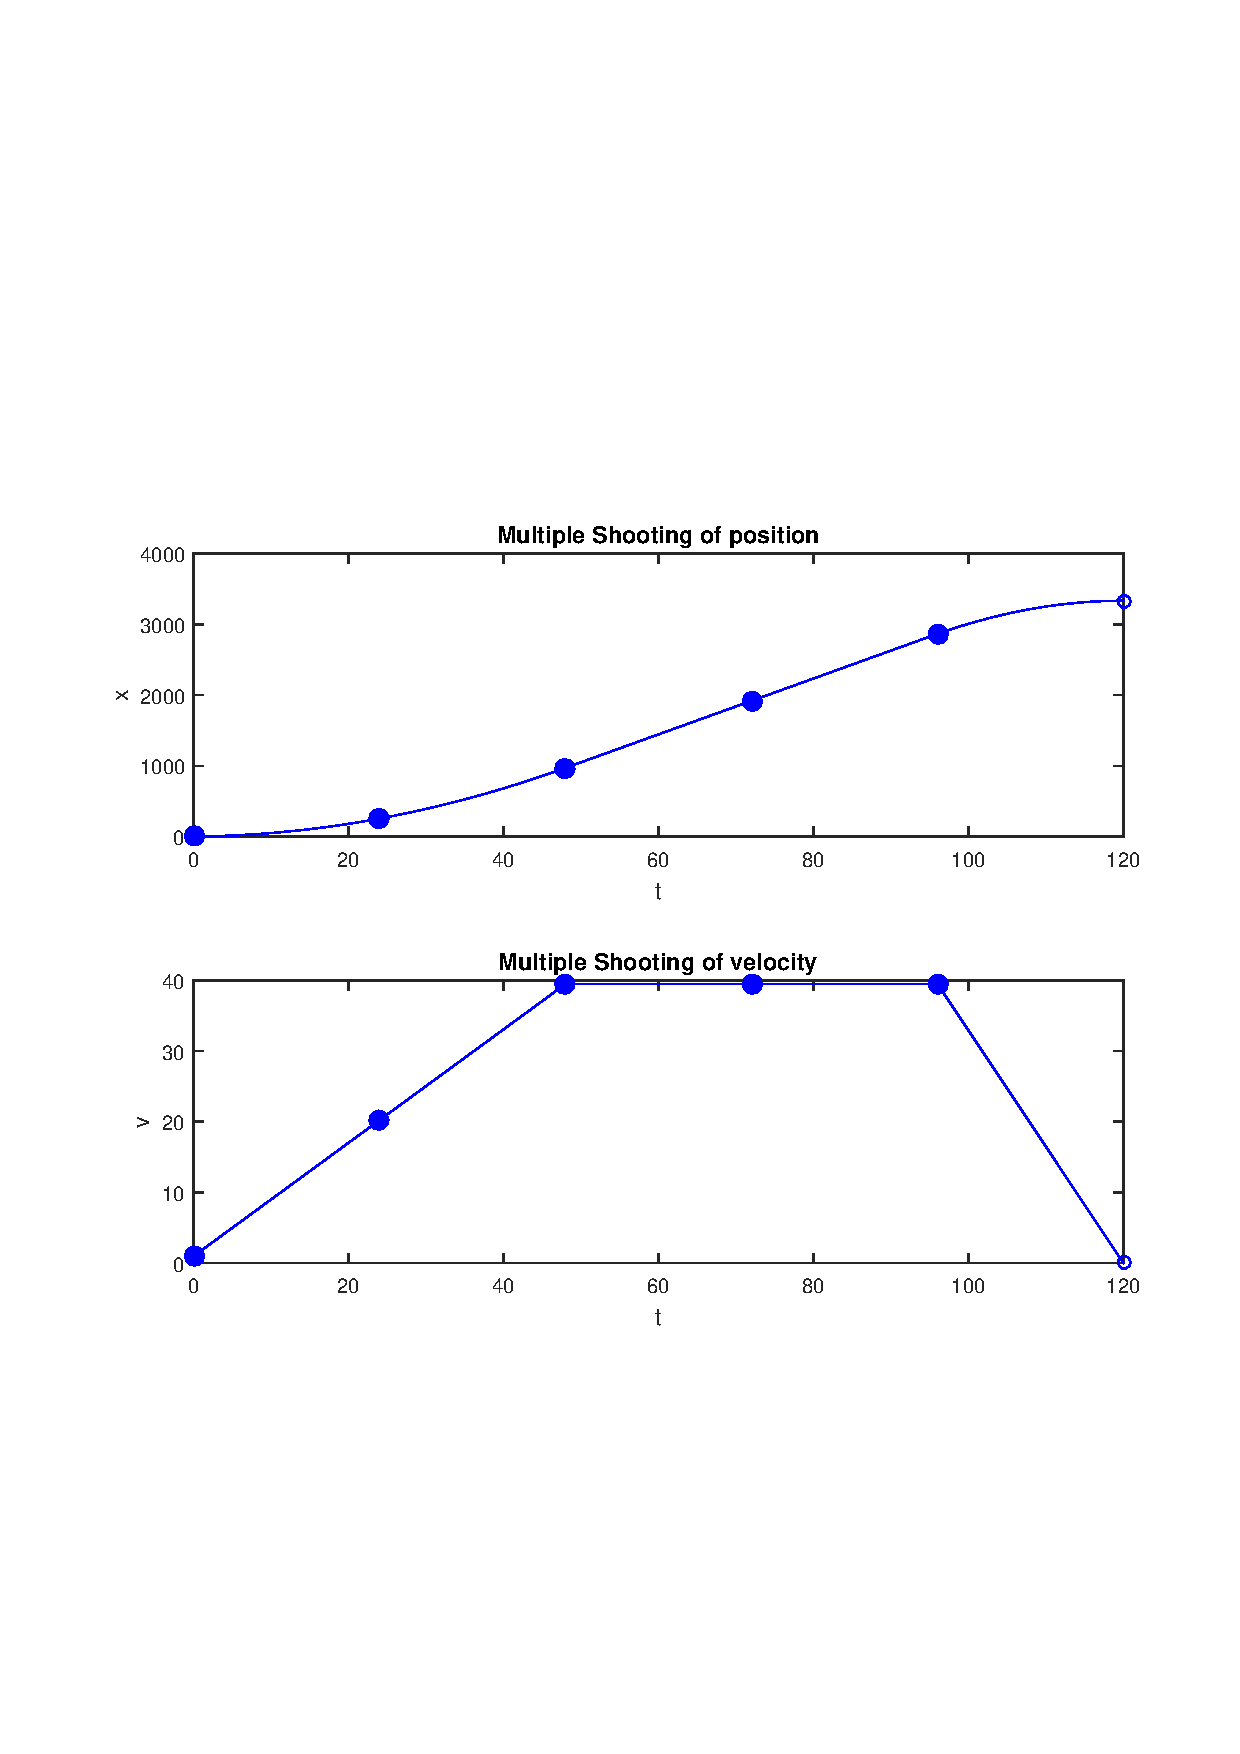
\includegraphics[width=0.9\textwidth]{Sabina/MultipleShooting27.pdf}
\end{figure}}
\only<6>{\begin{figure}
\centering
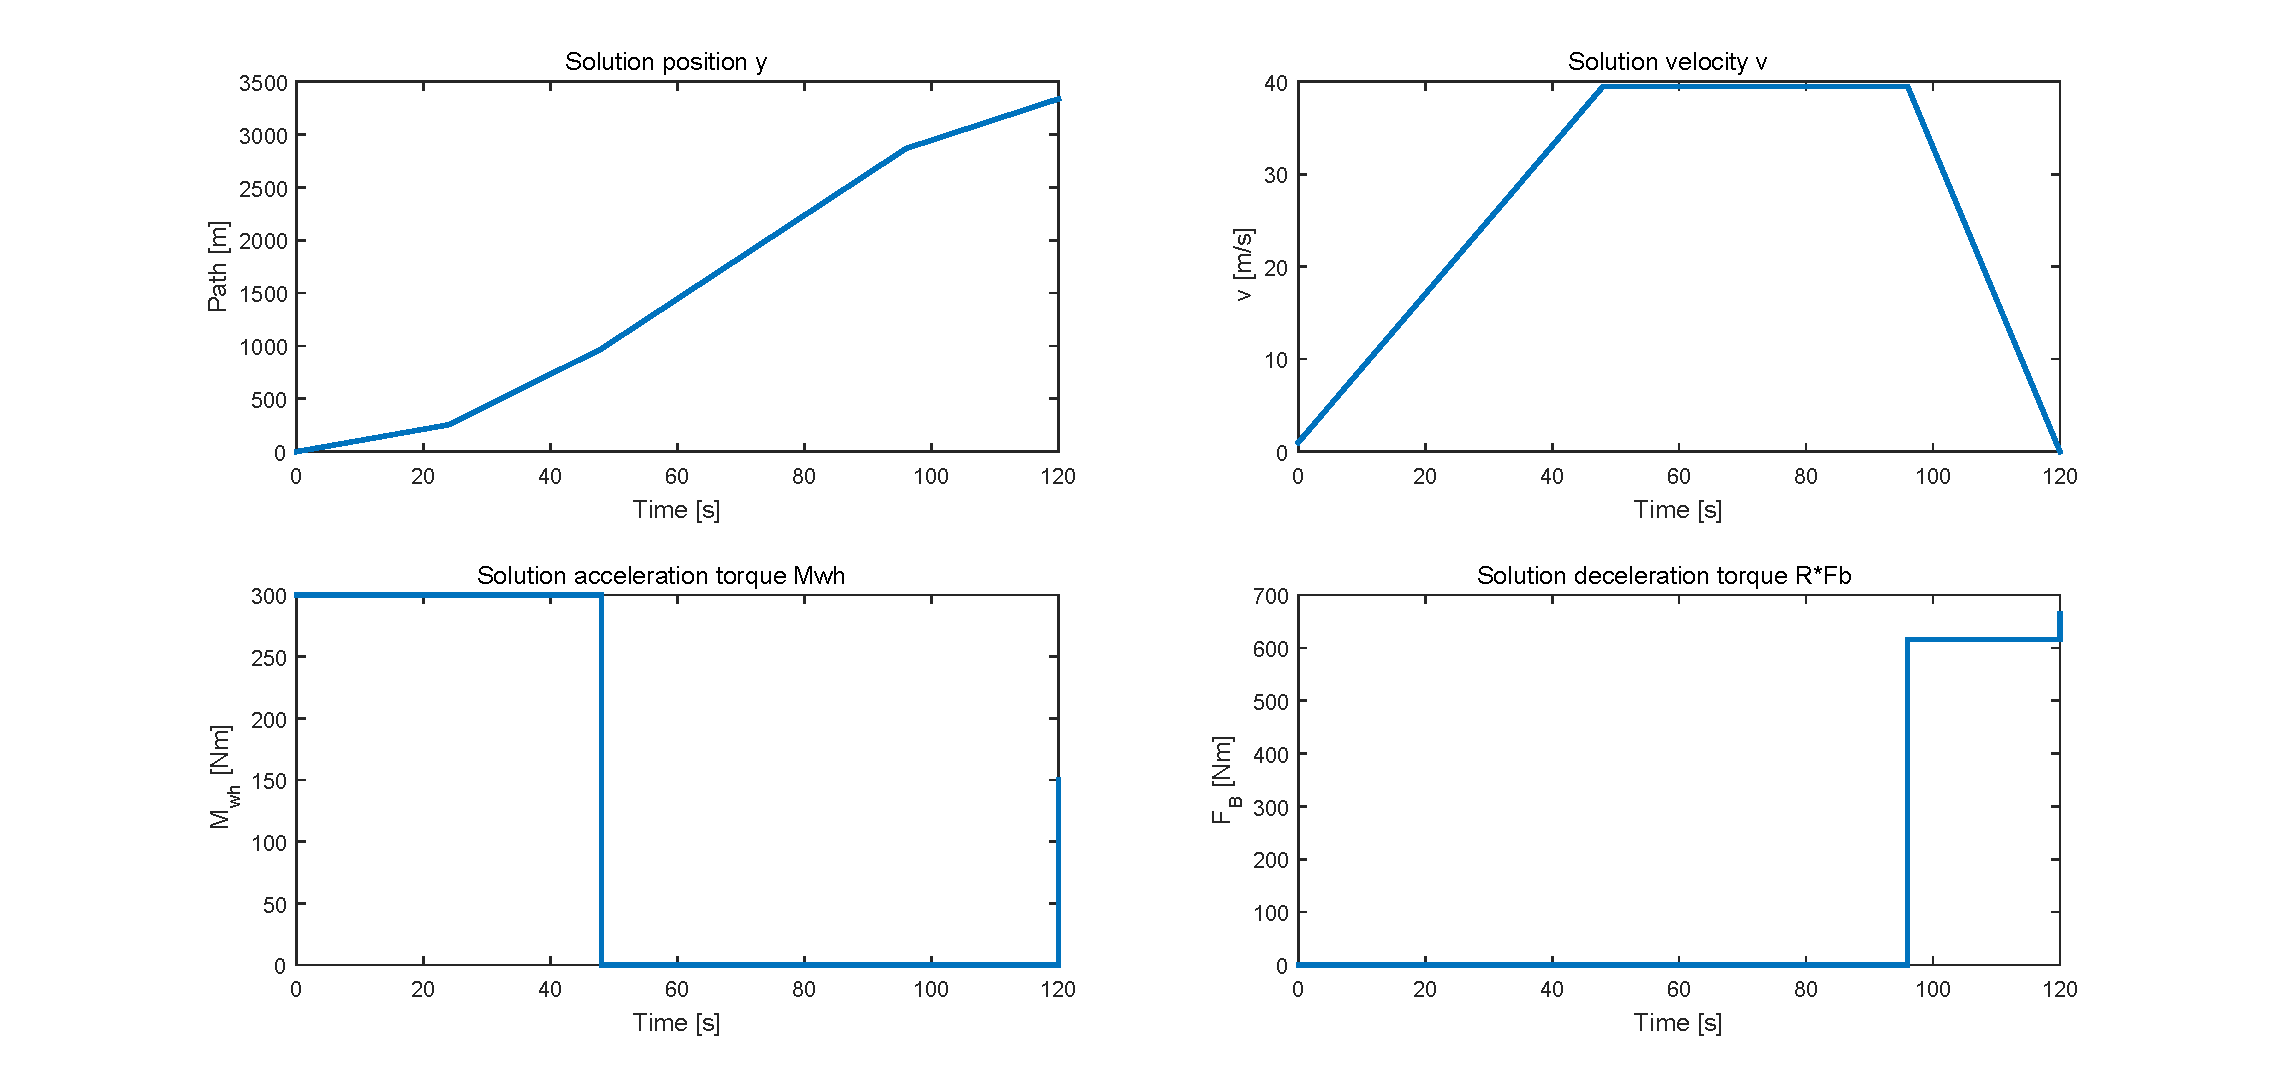
\includegraphics[width=1\textwidth]{Sabina/output.pdf}
\end{figure}}
\end{frame}